\documentclass{article}

% if you need to pass options to natbib, use, e.g.:
%     \PassOptionsToPackage{numbers, compress}{natbib}
% before loading neurips_2018

% ready for submission
% \usepackage{neurips_2018}

% to compile a preprint version, e.g., for submission to arXiv, add add the
% [preprint] option:
%     \usepackage[preprint]{neurips_2018}

% to compile a camera-ready version, add the [final] option, e.g.:
     \usepackage[final]{neurips_2018}

% to avoid loading the natbib package, add option nonatbib:
%     \usepackage[nonatbib]{neurips_2018}

\usepackage[utf8]{inputenc} % allow utf-8 input
\usepackage[T1]{fontenc}    % use 8-bit T1 fonts
\usepackage{hyperref}       % hyperlinks
\usepackage{url}            % simple URL typesetting
\usepackage{booktabs}       % professional-quality tables
\usepackage{amsfonts}       % blackboard math symbols
\usepackage{nicefrac}       % compact symbols for 1/2, etc.
\usepackage{microtype}      % microtypography
\usepackage{float}
\usepackage{graphicx}

\title{Project S Proposal}

% The \author macro works with any number of authors. There are two commands
% used to separate the names and addresses of multiple authors: \And and \AND.
%
% Using \And between authors leaves it to LaTeX to determine where to break the
% lines. Using \AND forces a line break at that point. So, if LaTeX puts 3 of 4
% authors names on the first line, and the last on the second line, try using
% \AND instead of \And before the third author name.

\author{%
  Xin Chen, Yun Yeong Choi  \\
  Department of Materials Science and Engineering\\
  University of California, Berkeley\\
%   Berkeley, CA 94720-1760 \\
  \texttt{\{chenxin0210, yychoi94\}@berkeley.edu} \\
  % examples of more authors
   \And
%   Yun Yeong Choi \\
%   Department of Materials Science and Engineering \\
%   University of California, Berkeley\\
%   \texttt{yychoi94@berkeley.edu} \\
%   \AND
   Ke Ma \\
   Department of Civil and Environment Engineering \\
   University of California, Berkeley \\
   \texttt{kema@berkeley.edu} \\
   \And
   Fengzhe Shi \\
   Department of Chemical Engineering \\
   University of California, Berkeley \\
   \texttt{schweini@berkeley.edu} \\
  % \And
  % Coauthor \\
  % Affiliation \\
  % Address \\
  % \texttt{email} \\
}

\begin{document}
% \nipsfinalcopy is no longer used

\maketitle


\section{Introduction}

Historically, many ancient astronomers were trying to predict the movement of the moon, planets, and stars for the purpose of astrology or agriculture. These kinds of efforts last for thousands of years and lead to the development of physics, from Newton's law of motion to Einstein's general relativity. 

In this project, we will focus to capture their efforts and inspiration by using machine learning techniques. In specific, we start from the old model and assumptions of ancient Chinese astronomers, such as Geocentrism. Based on the old model and modern observation data, we can identify how much the ancient model has deviated from the observations.

After that, we will try to mimic the human learning process by means of machine learning techniques. What the old astronomers did was looking into data long and deeply, and find out some equations and features that explain their data better. Instead of those painful and time-consuming process, what we are going to do in this project is to add possible features and fit them with data, choosing the most appropriate features which make models better using machine learning techniques. Start from the ancient one, we will develop our own model and predict the movement of stellar bodies based on these machine-learned models. Also, our final goal is to find the features that made great improvement, and explain what is the physics behind these features.

\section{Ancient Chinese Astronomy Theories}
What is the meaning of the shining stars high up in the night sky? Ancient Chinese have been looking into the sky for the answer, for thousands of years. Lots of theories were proposed and developed throughout history, and in the third century AD, the ideas converged into 3 main theories, i.e. Gaitian, Huntian, and Xuanye, as concluded by Fang [1]. These theories are not completely isolated and share a lot of similar ideas, while also have disagreements over some key issues.

Gaitian was the most ancient theory that suggests that the sky is a geodesic dome, or a hemisphere covering the flat Earth. The theory claims that the sun is moving 80000 li (ancient Chinese lengthunit, 1li = 415.8m) above the Earth.

Huntian is a better-developed theory that claims the Earth to the sky is the yolk to the egg. In other words, the sky is a complete sphere where stars are attached to. The Earth is floating on water, which fills the bottom part of the sky sphere. The sky sphere rotates around the Earth around an axis 36degree to the horizontal direction. In the Huntian theory, the sun, the moon, and planets are special objects that revolve the Earth within the sky sphere, in a different direction.

Most part of Xuanye theory is lost in history while the remaining part claims that stars are not fixed into the so-called sky sphere. Instead, stars are believed to be floating in the air and moving at will. Such suggestions are based on the fact that some special stars (and planets) are not moving in the same patterns as other stellar objects are, even moving irregularly at times. Different from Huntian theory that uses special orbits to explain the movement of the planets, Xuanye claims all the stars and planets are not fixed to anything at all.

The theories themselves kept developing in order to fix problems and to better fit the observation. What we conclude here, especially the Huntian theory, is actually the result of generations of astronomers' hard work.

\section{Developing a Mathematical Model}
Based on the most fundamental rule of Huntian theory, the earth is fixed in the center of the universe while all other stars, planets, the sun, and the moon orbit around it. We will respect this basic premise and re-develop our model on it.

% We are going to give a quantitative explanation to this theory by training a model with modern datasets.
In detail, since the basic idea is to fit such an ancient model, we will feed the model with featurized modern data such as time and position of stellar bodies according to an Earth observer, just the same coordinate system as what an ancient astronomer would use by looking directly into the sky.

%In order to see how the phenomenons will be regarding the time and location on Earth, we first need data to represent celestial objects. 

%The data we feed the model would be mainly positions of different objects in space from an Earth observer, the observation time, etc. Considering the structure of Huntian Theory, we need to do feature engineering to fit this model. We would probably need to use features so that our model has a circular orbit. Unlike modern theory, Huntian Theory treats the Earth as the center of universe and doesn't consider the facts of the changeable velocity, relative positions, etc. of the astronomical objects. 

In general, similar to how ancient astronomers developed their theories, we will start from the most basic Huntian theory, i.e. an Earth-centered model with everything else orbiting it in a similar pattern. By ruling out exceptions and adding features accordingly, we will then develop the theory to fit the observation better.

For example, the retrograde motion of planets [2] is extremely hard to be predicted by this Earth-centered model, if without appropriate features. In that case, we will have to introduce additional features to fit the observation better.

\begin{figure}[H]
    \centering
    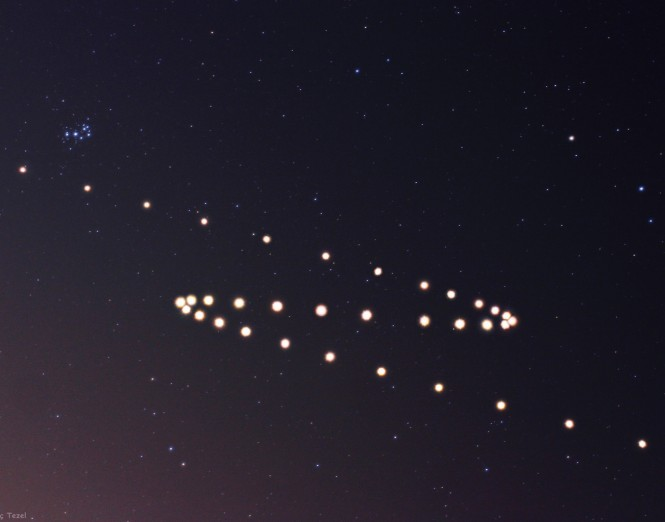
\includegraphics[width=8cm]{mars.jpg}
    \caption{Retrograde motion of mars - 2013}
    \label{fig:mars}
\end{figure}

The goals of the project require the model to be able to make predictions in two parts. One is the positions of the planets, the moon, and the sun based on the time and position on the Earth. In this case, we would construct the training set as $(X_i, y_i)$ pairs, where $X_i$ would contain the time and the position of the Earth and $y_i$ is a matrix containing the positions of the stellar body $i$. We will featurize $X_i$ into $\phi(X_i)$ and several features will be tested and updated by training our model. Should different features show a similar error, we will choose more simple features for our model to maintaining simplicity. %and to connect with real theory.

The other goal is to make predictions on the eclipses and the phase of the moon based on the time and positions on the Earth. In this case study, $X_i$ would be the same while $y_i$ would be vectors that could describe the eclipses and the phase of the moon. %We would use different numbers to denote those phenomena. 

Considering the restriction of science and technology in ancient times, Huntian Theory is already an advanced model, but there are still a lot of defects. Xuanye Theory, to some extent, compensates for the drawbacks of Huntian theory, which unfortunately has been lost in the long history of humanity. In a possible further development, we will try to build our own model to include the core idea of Xuanye Theory. By collecting clues from ancient books, we hope to remedy the missing fragment of history with the modern tool of machine learning. 

\section*{References}

\medskip

\small

[1] Fang, X. (1974). Jin shu. Beijing: Zhonghua shu ju.

[2] Bruce G. Thompson.\ (2005) Using retrograde motion to understand and determine orbital parameters. {\it American Journal of Physics 73, 1023}

\end{document}